\documentclass[a4paper, 12pt]{article}

\usepackage[margin=2.3cm]{geometry}
\usepackage[utf8]{inputenc}
\usepackage{float}
\usepackage{xcolor}
\usepackage{amsmath}
\usepackage{graphicx}
\usepackage{hyperref}

\definecolor{darkblue}{rgb}{0.21, 0.60, 0.86}
\definecolor{darkgreen}{rgb}{0.15, 0.68, 0.38}
\definecolor{darkorange}{rgb}{0.83, 0.33, 0}
\definecolor{darkyellow}{rgb}{0.95, 0.77, 0.06}
\definecolor{darkred}{rgb}{0.91, 0.29, 0.24}

\newcommand{\bc}[2]{\textbf{\textcolor{#1}{#2}}}

\graphicspath{ {images/} }
\setlength{\parindent}{0pt}

\title{Docker Documentation}
\author{Kyle Chapman}
\date{February 2020}

\begin{document}

\maketitle
\tableofcontents
\clearpage

\section{Structure}

\begin{figure}[H]
	\centering
	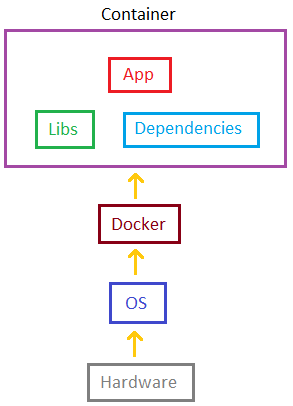
\includegraphics[scale=0.6]{docker-setup.png}
	\caption{Structure of Docker}
\end{figure}

A \texttt{Dockerfile} is used to create images, and an image is used to deploy
an application. A container only lives as long as the process inside it is
alive.

\section{Dockerfile Format}

Given the following \texttt{Dockerfile}:

\begin{verbatim}
1.  FROM ubuntu
2.
3.  RUN apt-get update
4.  RUN apt-get install python
5.
6.  RUN pip install flask
7.
8.  COPY . ~/Desktop/Project/docker-files
9.
10. ENTRYPOINT FLASK_APP=~/Desktop/Project/docker-files/app.py flask run
\end{verbatim}

\textbf{Note}:
\begin{itemize}
	\item All words in \texttt{CAPS} are \bc{darkorange}{instructions} and all
	other words represent the \bc{darkyellow}{arguments}.
	\item Every docker image must be based on another image and the
	\texttt{Dockerfile} must start with \texttt{FROM}.
	\item \texttt{COPY} copies files from the local storage onto the Docker
	container.
	\item \texttt{ENTRYPOINT} specifies a command that must be run when starting
	the image in the Docker container.
	\item All \bc{darkyellow}{arguments} are stored in cache so that if you
	re-run the \texttt{docker build} command, you don`t need to re-download the
	necessary files.
\end{itemize}

Given the following \texttt{Dockerfile}:
\begin{verbatim}
1.  FROM ubuntu
2.
3.  ENTRYPOINT ["sleep"]
4.
5.  CMD ["5"]
\end{verbatim}

When running \texttt{docker run <appName> <sleepMilli>} with no value given for
\texttt{sleepMilli}, a default value of \texttt{5} will be used as specified
by \texttt{CMD}. Otherwise, any value entered for \texttt{sleepMilli} will
replace the \texttt{5}.

\section{Networking}

\begin{figure}[H]
	\centering
	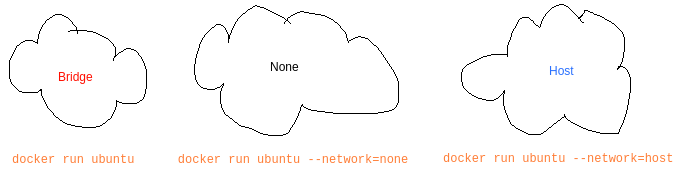
\includegraphics[scale=0.5]{network.png}
\end{figure}

\section{Commands}

Prefix all the following commands with \texttt{\bc{darkblue}{docker}}:

\subsection{ps}

Lists all the running containers.

\vspace{0.5em}
Examples:
\begin{itemize}
	\item \texttt{ps} $\Rightarrow$ List all the running containers.
	\item \texttt{ps -a} $\Rightarrow$ List all containers that are currently
	running or have exited.
\end{itemize}

\subsection{history}

Shows all the instructions that were executed as a result of building the image.

\vspace{0.5em}
Example:
\begin{itemize}
	\item \texttt{history <hubUsername>/<appName>} $\Rightarrow$ Shows the
	layers executed by building the image \texttt{appName}.
\end{itemize}

\subsection{build}

Builds a docker image using settings from the \texttt{Dockerfile} configuration
file.

\vspace{0.5em}
Example:
\begin{itemize}
	\item \texttt{build <Dockerfile> -t <hubUsername>/<appName>} $\Rightarrow$
	Builds a docker image called \texttt{appName} using the configuration found
	in the \texttt{Dockerfile}.
\end{itemize}

\subsection{run}

Starts a docker container with the given image, downloading the image if not
already present.

\vspace{0.5em}
Examples:
\begin{itemize}
	\item \texttt{run <imageName>} $\Rightarrow$ Runs a specific image
	in a docker container.
	\item \texttt{run <imageName>:<versionNumber>} $\Rightarrow$ Runs a specific
	image with a specific version number. If no version number is provided,
	defaults to the latest version.
	\item \texttt{run -d <imageName>} $\Rightarrow$ Runs a specific image in a
	detached state, i.e. no console output. See \ref{sec:attach} to see console
	output.
	\item \texttt{run -p <externalPort>:<internalPort> <imageName>}
	$\Rightarrow$ Runs a specific image and binds an external port to an
	internal port, so that users outside of the docker host can access the app
	using the \texttt{externalPort}, which would redirect to the
	\texttt{internalPort} inside the docker host.
	\item \texttt{run -v <localDir>:<dockerDir> <imageName>} $\Rightarrow$ Runs
	a specific image and persists all changes to the \texttt{dockerDir}
	directory to the \texttt{localDir} directory.
	\item \texttt{run -it <imageName>} $\Rightarrow$ Runs a specific image in
	interactive mode (\texttt{-i}) with a pseudo-terminal (\texttt{-t}),
	allowing for user input.
\end{itemize}

\subsection{stop}

Stops the running container that matches the container ID.

\vspace{0.5em}
Example:
\begin{itemize}
	\item \texttt{stop <containerID>} $\Rightarrow$ Stops the container that
	matches the container ID.
\end{itemize}

\subsection{rm}

Removes a container that matches the container ID.

\vspace{0.5em}
Example:
\begin{itemize}
	\item \texttt{rm <containerID>} $\Rightarrow$ Removes the container that
	matches the container ID from the local file system.
\end{itemize}

\subsection{rmi}

Removes an image that matches the image name.

\vspace{0.5em}
Example:
\begin{itemize}
	\item \texttt{rmi <imageName>} $\Rightarrow$ Remove a specific image that
	has been downloaded.
\end{itemize}

\subsection{images}

Shows all of the downloaded docker images.

\subsection{pull}

Download a specific docker image from docker hub.

\vspace{0.5em}
Example:
\begin{itemize}
	\item \texttt{pull <imageName>} $\Rightarrow$ Download the image with the
	matching image name.
\end{itemize}

\subsection{exec}

Executes a command on a docker container.

\vspace{0.5em}
Example:
\begin{itemize}
	\item \texttt{exec <containerID> <command>} $\Rightarrow$ Executes a
	specific command on the matching container ID, where \texttt{<command>} can
	be \texttt{ls -la} as an example.
\end{itemize}

\subsection{\label{sec:attach}attach}

Attaches the console to the container ID specified.

\vspace{0.5em}
Example:
\begin{itemize}
	\item \texttt{attach <containerID>} $\Rightarrow$ Attach a console to the
	container ID specified.
\end{itemize}

\subsection{inspect}

Shows detailed information about the container specified.

\vspace{0.5em}
Example:
\begin{itemize}
	\item \texttt{inspect <containerID>} $\Rightarrow$ Show detailed information
	about the container with the matching ID.
\end{itemize}

\subsection{logs}

Shows the logs of the container that has been specified.

\vspace{0.5em}
Example:
\begin{itemize}
	\item \texttt{logs <containerID>} $\Rightarrow$ Show logs for container
	with matching ID.
\end{itemize}

\subsection{push}

Pushes a generated Docker image to the Docker hub.

\vspace{0.5em}
Example:
\begin{itemize}
	\item \texttt{push <hubUsername>/<appName>} $\Rightarrow$ Pushes the
	generated image to Docker hub with the name \texttt{appName}.
\end{itemize}

\end{document}
